%\documentclass[conference]{IEEEtran}
\newcommand{\CLASSINPUTinnersidemargin}{25mm}
\newcommand{\CLASSINPUTtoptextmargin}{20mm}
\documentclass[12pt,onecolumn,technote]{IEEEtran}
\IEEEoverridecommandlockouts
\usepackage{cite}
\usepackage{amsmath,amssymb,amsfonts}
\usepackage{algorithmic}
\usepackage{graphicx}
\usepackage{textcomp}
\usepackage{polski}
\usepackage[utf8]{inputenc}
\usepackage{xcolor}
\def\BibTeX{{\rm B\kern-.05em{\sc i\kern-.025em b}\kern-.08em
    T\kern-.1667em\lower.7ex\hbox{E}\kern-.125emX}}
\begin{document}
\Large
\title{MSI Projekt}

\author{\IEEEauthorblockN{Jakub Cembrzyński}
\IEEEauthorblockA{\textit{235544}}\\
\and
\IEEEauthorblockN{Oskar Kowalik}
\IEEEauthorblockA{\textit{235349}}\\
\and
\IEEEauthorblockN{Szymon Sakowicz}
\IEEEauthorblockA{\textit{235249}}\\
\and
}

\maketitle

\begin{abstract}
Naukowy projekt grupowy mający na celu zbadanie wpływu metody random subspace na dokładność klasyfikatorów. Eksperyment został wykonany w ramach zajęć "Metody sztucznej inteligencji".
\end{abstract}
\large

\section{Wybór dowolnego algorytmu klasyfikacji, regresji, segmentacji lub preprocessingu,
}
W przypadku uczenia maszynowego mamy do czynienia z uczeniem dzielącym się na nadzorowane i nienadzorowane oraz testowaniem tworzonego przez nas klasyfikatora. Problem klasyfikacji na którym postanowiliśmy się skupić polega na przypisaniu badanych obiektów do odpowiednich grup reprezentujących podobne cechy.


W naszej pracy wykorzystaliśmy następujące algorytmy klasyfikacji:
\subsection{kNN - k najbliższych sąsiadów}
K najbliższych sąsiadów jest jednym z algorytmów regresji nieparametrycznej używanym do prognozowania wartości pewnej zmiennej losowej. Można go zastosować do klasyfikacji. Korzysta on z tak zwanego uczenia leniwego, więc jest on dość kosztowny obliczeniowo, jednakże jest prosty algorytmicznie. Predykcja składa się tylko z dwóch kroków: znajdź k  najbliższych sąsiadów, zwróć najczęstszą ich etykietę. Przy używaniu tego algorytmu należy pamiętać o prawidłowym dobraniu parametru k, tak, aby nie było zbyt małe, aby obserwacje odstające nie wpływały znacząco na wynik; oraz zbyt duże, aby nie uprościć klasyfikacji do wyboru klasy dominującej według prawdopodobieństwa a priori.
\subsection{Gaussowski naiwny Bayes}
Gaussowski naiwny Bayes jest prostym klasyfikatorem probabilistycznym. Wylicza prawdopodobieństwo a posteriori na podstawie prawdopodobieństwa a priori. Oparty jest na założeniu, iż wpływ cech na na prawdopodobieństwa przynależności do klas jest niezależny, choć często jest.
\subsection{Drzewo decyzyjne}
Klasyfikacja za pomocą drzewa decyzyjnego polega na przejściu po kolejnych testach zwanych węzłami, idąc od korzeni do liści. Osiągnięcie liścia wyznacza kategorię, w ten sposób można zaklasyfikować dowolny przykład.
\subsection{SVC}
Klasyfikator SVC służy do klasyfikacji binarnej. Szuka optymalnej płaszczyzny poprawnie oddzielającej klasyfikowane obiekty szukając mającej przy tym najwyższy margines separacji. Pozwala to poprawnie sklasyfikować badane obiekty oraz zminimalizować ryzyko popełnienia pomyłki dla nowych obiektów.


\section{Wybór adekwatnych danych testowych}

Do badania wykorzystaliśmy udostępnione nam zbiory danych składające się z cech obiektów i przypisanych im etykiet. Zgodnie z założeniami random subspace wiedza o danych w zbiorach jest zbędna z punktu widzenia eksperymentu. Wszystkie wykorzystane zbiory są zbiorami binarnymi. Oznacza to, że wartości w kolumnie przechowującej etykiety wynosi 0 lub 1, a klasyfikator przyporządkowuje obiekty do dwóch grup.

\vspace{12pt}
\begin{table}[h]
    \large
    \caption{Liczność naszego zbioru danych}
    \begin{tabular}{|p{0.25\linewidth}|p{0.25\linewidth}|p{0.25\linewidth}|p{0.25\linewidth}|}
\hline
     \textbf{Zbiór danych} & \textbf{Liczba obiektów} & \textbf{Liczba cech} & \textbf{Liczba klas} \\
\hline
     \textbf{Diabetes} & 768 & 8 & 2 \\
\hline
     \textbf{Wine} & 178 & 13 & 2 \\
\hline
     \textbf{German} & 1000 & 24 & 2 \\
\hline
     \textbf{POPfailures} & 540 & 20 & 2 \\
\hline
     \textbf{Heart} & 270 & 13 & 2 \\
\hline
     \textbf{Liver} & 345 & 6 & 2 \\
\hline
\end{tabular}
\end{table}
\vspace{12pt}


\section{Wprowadzenie autorskiej modyfikacji w wybranym algorytmie i implementacja jako poprawnego estymatora scikit-learn}

Każdy z wyżej wymienionych klasyfikatorów został zaimplementowany na nowo przy użyciu biblioteki scikit-learn. W celu poprawienia dokładności powyższych klasyfikatorów postanowiliśmy wykorzystać metodę random subspace (losowych podzbiorów generowanych z dostępnych zbiorów danych). Każdy z klasyfikatorów został wyuczony przy pomocy powstałych podzbiorów. Eksperyment został przeprowadzony dla różnej ilości generowanych podzbiorów.

\section{Wybór standardowych metod porównawczych}

W naszym eksperymencie zdecydowaliśmy się skorzystać z dokładności jako metody porównawczej pomiędzy wynikami dla klasyfikatorów domyślnych i z zastosowaniem random subspace. Dla każdego klasyfikatora przeprowadzana określona liczba testów poprawności dla danego zbioru oraz tworzony jest zbiór etykiet przypisanych przez klasyfikator. Następnie sprawdzamy ile etykiet zostało poprawnie przypisanych przez algorytm wyuczony pełnym zbiorem podzielonym na zbiór uczący i testowy oraz przez algorytm wytrenowany na bazie podzbiorów. Jako skuteczniejszy klasyfikator wybierany jest ten, który więcej razy osiągnął wyższą dokładność.

\section{Konstrukcja i przeprowadzenie eksperymentów}

W pierwszej części projektu zbiory z pominiętymi etykietami zostały podzielone na zbiory uczące i testowe w proporcji 70:30. Przy ich pomocy wyuczyliśmy wybrane przez nas algorytmy, a następnie przetestowaliśmy ich działanie zapamiętując przy tym przypisane obiektom etykiety.

Następnie dla zmiennej ilości podzbiorów i ich rozmiarów przeprowadziliśmy od nowa wyuczenie klasyfikatorów oraz testowanie ich przy pomocy wygenerowanych podzbiorów.

Na końcu sprawdzamy dokładność algorytmów wytrenowanych w pierwszej części eksperymentu oraz tych wytrenowanych przy użyciu losowych podzbiorów. Metoda z wyższym wynikiem zostaje uznana za dokładniejszą.

\section{Analiza statystyczna wyników}
Przy zastosowaniu zbioru uczącego podzielonego na zbiór uczący i testowy otrzymaliśmy następujące wyniki.
Dla klasyfikatorów wyuczonych przy pomocy podzbiorów dokładność wzrosła w stosunku do domyślnego klasyfikatora. 
Poniższy wykres przedstawia wpływ liczby wygenerowanych podzbiorów na dokładność klasyfikatora wyuczonego przy ich pomocy względem domyślnego.


\newpage
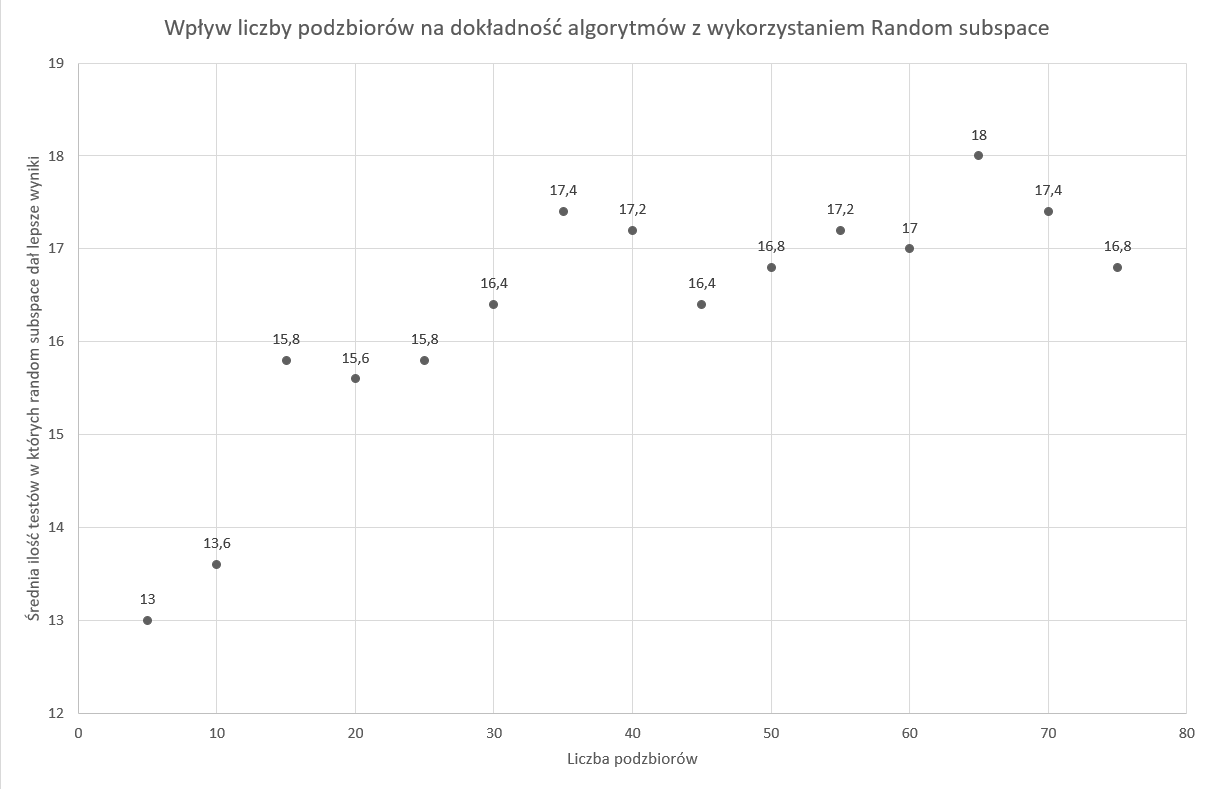
\includegraphics[height=\textwidth,width=24cm,angle=90]{wykres.png}
\newpage


Wartości na wykresie to wartości średnie z pięciu testów dla każdej liczby wykorzystanych podzbiorów. Wykres pokazuje nam, że już przy pięciu podzbiorach zastosowanie metody random subspace daje lepsze wyniki niż przy jej braku. Wraz ze wzrostem liczby podzbiorów dokładność rośnie. Przy liczbie 15 podzbiorów można zauważyć dość znaczącą liczbę testów z lepszymi wynikami. Można zauważyć, że wystaczy około 30 podzbiorów, aby ilość testów z lepszymi wynikami ustabilizowała się mniej więcej na tym samym poziomie. 

Najlepsze wyniki zostały uzyskane dla 35 oraz 65 podzbiorów. Z uwagi na spory koszt obliczeniowy przy większej liczbie podzbiorów oraz za małe uczenie przy małej liczbie podzbiorów możemy wysunąć wniosek, iż najbardziej optymalną liczbą podzbiorów dla badanych zbiorów danych jest 35.

\section{Redakcja pracy}

\begin{thebibliography}{00}
\bibitem{b1} Daniel Hnyk. (2019). Creating your own estimator in scikit-learn. http://danielhnyk.cz/creating-your-own-estimator-scikit-learn/ [23 Maj 2019].
\bibitem{b2} Ksieniewicz, P. (2019). Metody Sztucznej Inteligencji - Wykład 1: Historia i podstawowe pojęcia. 
\bibitem{b3} Ksieniewicz, P. (2019). Metody Sztucznej Inteligencji - Wykład 2: Zadanie klasyfikacji
\bibitem{b4} Ksieniewicz, P. (2019). Metody Sztucznej Inteligencji - Wykład 3: Już nie leniwe, ale naiwne. 
\bibitem{b5} Ksieniewicz, P. (2019). Metody Sztucznej Inteligencji - Wykład 4: Projektowanie eksperymentów oceniających jakość klasyfikacji
\bibitem{b6} Pl.wikipedia.org. (2019). K najbliższych sąsiadów. https://pl.wikipedia.org/wiki/K\_najbliższych\_sąsiadów [23 Maj 2019].
\bibitem{b7} Pl.wikipedia.org. (2019). Naiwny klasyfikator bayesowski https://pl.wikipedia.org/wiki/Naiwny\_klasyfikator\_bayesowski [23 Maj 2019].
\bibitem{b8} Wazniak.mimuw.edu.pl. (2019). Sztuczna inteligencja/SI Moduł 10 - Zadanie i metody klasyfikacji - 
Studia Informatyczne. http://wazniak.mimuw.edu.pl/index.php?title=Sztuczna\_inteligencja/SI\_Moduł\_10\_-\_Zadanie\_i\_metody\_klasyfikacji [23 Maj 2019].
\end{thebibliography}
\end{document}
